%% bare_jrnl.tex
%% V1.4b
%% 2015/08/26
%% by Michael Shell
%% see http://www.michaelshell.org/
%% for current contact information.
%%
%% This is a skeleton file demonstrating the use of IEEEtran.cls
%% (requires IEEEtran.cls version 1.8b or later) with an IEEE
%% journal paper.
%%
%% Support sites:
%% http://www.michaelshell.org/tex/ieeetran/
%% http://www.ctan.org/pkg/ieeetran
%% and
%% http://www.ieee.org/

%%*************************************************************************
%% Legal Notice:
%% This code is offered as-is without any warranty either expressed or
%% implied; without even the implied warranty of MERCHANTABILITY or
%% FITNESS FOR A PARTICULAR PURPOSE! 
%% User assumes all risk.
%% In no event shall the IEEE or any contributor to this code be liable for
%% any damages or losses, including, but not limited to, incidental,
%% consequential, or any other damages, resulting from the use or misuse
%% of any information contained here.
%%
%% All comments are the opinions of their respective authors and are not
%% necessarily endorsed by the IEEE.
%%
%% This work is distributed under the LaTeX Project Public License (LPPL)
%% ( http://www.latex-project.org/ ) version 1.3, and may be freely used,
%% distributed and modified. A copy of the LPPL, version 1.3, is included
%% in the base LaTeX documentation of all distributions of LaTeX released
%% 2003/12/01 or later.
%% Retain all contribution notices and credits.
%% ** Modified files should be clearly indicated as such, including  **
%% ** renaming them and changing author support contact information. **
%%*************************************************************************


% *** Authors should verify (and, if needed, correct) their LaTeX system  ***
% *** with the testflow diagnostic prior to trusting their LaTeX platform ***
% *** with production work. The IEEE's font choices and paper sizes can   ***
% *** trigger bugs that do not appear when using other class files.       ***                          ***
% The testflow support page is at:
% http://www.michaelshell.org/tex/testflow/



\documentclass[journal]{IEEEtran}
%
% If IEEEtran.cls has not been installed into the LaTeX system files,
% manually specify the path to it like:
% \documentclass[journal]{../sty/IEEEtran}





% Some very useful LaTeX packages include:
% (uncomment the ones you want to load)


% *** MISC UTILITY PACKAGES ***
%
%\usepackage{ifpdf}
% Heiko Oberdiek's ifpdf.sty is very useful if you need conditional
% compilation based on whether the output is pdf or dvi.
% usage:
% \ifpdf
%   % pdf code
% \else
%   % dvi code
% \fi
% The latest version of ifpdf.sty can be obtained from:
% http://www.ctan.org/pkg/ifpdf
% Also, note that IEEEtran.cls V1.7 and later provides a builtin
% \ifCLASSINFOpdf conditional that works the same way.
% When switching from latex to pdflatex and vice-versa, the compiler may
% have to be run twice to clear warning/error messages.






% *** CITATION PACKAGES ***
%
%\usepackage{cite}
% cite.sty was written by Donald Arseneau
% V1.6 and later of IEEEtran pre-defines the format of the cite.sty package
% \cite{} output to follow that of the IEEE. Loading the cite package will
% result in citation numbers being automatically sorted and properly
% "compressed/ranged". e.g., [1], [9], [2], [7], [5], [6] without using
% cite.sty will become [1], [2], [5]--[7], [9] using cite.sty. cite.sty's
% \cite will automatically add leading space, if needed. Use cite.sty's
% noadjust option (cite.sty V3.8 and later) if you want to turn this off
% such as if a citation ever needs to be enclosed in parenthesis.
% cite.sty is already installed on most LaTeX systems. Be sure and use
% version 5.0 (2009-03-20) and later if using hyperref.sty.
% The latest version can be obtained at:
% http://www.ctan.org/pkg/cite
% The documentation is contained in the cite.sty file itself.






% *** GRAPHICS RELATED PACKAGES ***
%
\ifCLASSINFOpdf
  % \usepackage[pdftex]{graphicx}
  % declare the path(s) where your graphic files are
  % \graphicspath{{../pdf/}{../jpeg/}}
  % and their extensions so you won't have to specify these with
  % every instance of \includegraphics
  % \DeclareGraphicsExtensions{.pdf,.jpeg,.png}
\else
  % or other class option (dvipsone, dvipdf, if not using dvips). graphicx
  % will default to the driver specified in the system graphics.cfg if no
  % driver is specified.
  % \usepackage[dvips]{graphicx}
  % declare the path(s) where your graphic files are
  % \graphicspath{{../eps/}}
  % and their extensions so you won't have to specify these with
  % every instance of \includegraphics
  % \DeclareGraphicsExtensions{.eps}
\fi
% graphicx was written by David Carlisle and Sebastian Rahtz. It is
% required if you want graphics, photos, etc. graphicx.sty is already
% installed on most LaTeX systems. The latest version and documentation
% can be obtained at: 
% http://www.ctan.org/pkg/graphicx
% Another good source of documentation is "Using Imported Graphics in
% LaTeX2e" by Keith Reckdahl which can be found at:
% http://www.ctan.org/pkg/epslatex
%
% latex, and pdflatex in dvi mode, support graphics in encapsulated
% postscript (.eps) format. pdflatex in pdf mode supports graphics
% in .pdf, .jpeg, .png and .mps (metapost) formats. Users should ensure
% that all non-photo figures use a vector format (.eps, .pdf, .mps) and
% not a bitmapped formats (.jpeg, .png). The IEEE frowns on bitmapped formats
% which can result in "jaggedy"/blurry rendering of lines and letters as
% well as large increases in file sizes.
%
% You can find documentation about the pdfTeX application at:
% http://www.tug.org/applications/pdftex





% *** MATH PACKAGES ***
%
\usepackage{amsmath}
% A popular package from the American Mathematical Society that provides
% many useful and powerful commands for dealing with mathematics.
%
% Note that the amsmath package sets \interdisplaylinepenalty to 10000
% thus preventing page breaks from occurring within multiline equations. Use:
%\interdisplaylinepenalty=2500
% after loading amsmath to restore such page breaks as IEEEtran.cls normally
% does. amsmath.sty is already installed on most LaTeX systems. The latest
% version and documentation can be obtained at:
% http://www.ctan.org/pkg/amsmath





% *** SPECIALIZED LIST PACKAGES ***
%
%\usepackage{algorithmic}
% algorithmic.sty was written by Peter Williams and Rogerio Brito.
% This package provides an algorithmic environment fo describing algorithms.
% You can use the algorithmic environment in-text or within a figure
% environment to provide for a floating algorithm. Do NOT use the algorithm
% floating environment provided by algorithm.sty (by the same authors) or
% algorithm2e.sty (by Christophe Fiorio) as the IEEE does not use dedicated
% algorithm float types and packages that provide these will not provide
% correct IEEE style captions. The latest version and documentation of
% algorithmic.sty can be obtained at:
% http://www.ctan.org/pkg/algorithms
% Also of interest may be the (relatively newer and more customizable)
% algorithmicx.sty package by Szasz Janos:
% http://www.ctan.org/pkg/algorithmicx




% *** ALIGNMENT PACKAGES ***
%
%\usepackage{array}
% Frank Mittelbach's and David Carlisle's array.sty patches and improves
% the standard LaTeX2e array and tabular environments to provide better
% appearance and additional user controls. As the default LaTeX2e table
% generation code is lacking to the point of almost being broken with
% respect to the quality of the end results, all users are strongly
% advised to use an enhanced (at the very least that provided by array.sty)
% set of table tools. array.sty is already installed on most systems. The
% latest version and documentation can be obtained at:
% http://www.ctan.org/pkg/array


% IEEEtran contains the IEEEeqnarray family of commands that can be used to
% generate multiline equations as well as matrices, tables, etc., of high
% quality.




% *** SUBFIGURE PACKAGES ***
%\ifCLASSOPTIONcompsoc
%  \usepackage[caption=false,font=normalsize,labelfont=sf,textfont=sf]{subfig}
%\else
%  \usepackage[caption=false,font=footnotesize]{subfig}
%\fi
% subfig.sty, written by Steven Douglas Cochran, is the modern replacement
% for subfigure.sty, the latter of which is no longer maintained and is
% incompatible with some LaTeX packages including fixltx2e. However,
% subfig.sty requires and automatically loads Axel Sommerfeldt's caption.sty
% which will override IEEEtran.cls' handling of captions and this will result
% in non-IEEE style figure/table captions. To prevent this problem, be sure
% and invoke subfig.sty's "caption=false" package option (available since
% subfig.sty version 1.3, 2005/06/28) as this is will preserve IEEEtran.cls
% handling of captions.
% Note that the Computer Society format requires a larger sans serif font
% than the serif footnote size font used in traditional IEEE formatting
% and thus the need to invoke different subfig.sty package options depending
% on whether compsoc mode has been enabled.
%
% The latest version and documentation of subfig.sty can be obtained at:
% http://www.ctan.org/pkg/subfig

\usepackage{amssymb}
\usepackage{graphicx}


% *** FLOAT PACKAGES ***
%
%\usepackage{fixltx2e}
% fixltx2e, the successor to the earlier fix2col.sty, was written by
% Frank Mittelbach and David Carlisle. This package corrects a few problems
% in the LaTeX2e kernel, the most notable of which is that in current
% LaTeX2e releases, the ordering of single and double column floats is not
% guaranteed to be preserved. Thus, an unpatched LaTeX2e can allow a
% single column figure to be placed prior to an earlier double column
% figure.
% Be aware that LaTeX2e kernels dated 2015 and later have fixltx2e.sty's
% corrections already built into the system in which case a warning will
% be issued if an attempt is made to load fixltx2e.sty as it is no longer
% needed.
% The latest version and documentation can be found at:
% http://www.ctan.org/pkg/fixltx2e


%\usepackage{stfloats}
% stfloats.sty was written by Sigitas Tolusis. This package gives LaTeX2e
% the ability to do double column floats at the bottom of the page as well
% as the top. (e.g., "\begin{figure*}[!b]" is not normally possible in
% LaTeX2e). It also provides a command:
%\fnbelowfloat
% to enable the placement of footnotes below bottom floats (the standard
% LaTeX2e kernel puts them above bottom floats). This is an invasive package
% which rewrites many portions of the LaTeX2e float routines. It may not work
% with other packages that modify the LaTeX2e float routines. The latest
% version and documentation can be obtained at:
% http://www.ctan.org/pkg/stfloats
% Do not use the stfloats baselinefloat ability as the IEEE does not allow
% \baselineskip to stretch. Authors submitting work to the IEEE should note
% that the IEEE rarely uses double column equations and that authors should try
% to avoid such use. Do not be tempted to use the cuted.sty or midfloat.sty
% packages (also by Sigitas Tolusis) as the IEEE does not format its papers in
% such ways.
% Do not attempt to use stfloats with fixltx2e as they are incompatible.
% Instead, use Morten Hogholm'a dblfloatfix which combines the features
% of both fixltx2e and stfloats:
%
% \usepackage{dblfloatfix}
% The latest version can be found at:
% http://www.ctan.org/pkg/dblfloatfix




%\ifCLASSOPTIONcaptionsoff
%  \usepackage[nomarkers]{endfloat}
% \let\MYoriglatexcaption\caption
% \renewcommand{\caption}[2][\relax]{\MYoriglatexcaption[#2]{#2}}
%\fi
% endfloat.sty was written by James Darrell McCauley, Jeff Goldberg and 
% Axel Sommerfeldt. This package may be useful when used in conjunction with 
% IEEEtran.cls'  captionsoff option. Some IEEE journals/societies require that
% submissions have lists of figures/tables at the end of the paper and that
% figures/tables without any captions are placed on a page by themselves at
% the end of the document. If needed, the draftcls IEEEtran class option or
% \CLASSINPUTbaselinestretch interface can be used to increase the line
% spacing as well. Be sure and use the nomarkers option of endfloat to
% prevent endfloat from "marking" where the figures would have been placed
% in the text. The two hack lines of code above are a slight modification of
% that suggested by in the endfloat docs (section 8.4.1) to ensure that
% the full captions always appear in the list of figures/tables - even if
% the user used the short optional argument of \caption[]{}.
% IEEE papers do not typically make use of \caption[]'s optional argument,
% so this should not be an issue. A similar trick can be used to disable
% captions of packages such as subfig.sty that lack options to turn off
% the subcaptions:
% For subfig.sty:
% \let\MYorigsubfloat\subfloat
% \renewcommand{\subfloat}[2][\relax]{\MYorigsubfloat[]{#2}}
% However, the above trick will not work if both optional arguments of
% the \subfloat command are used. Furthermore, there needs to be a
% description of each subfigure *somewhere* and endfloat does not add
% subfigure captions to its list of figures. Thus, the best approach is to
% avoid the use of subfigure captions (many IEEE journals avoid them anyway)
% and instead reference/explain all the subfigures within the main caption.
% The latest version of endfloat.sty and its documentation can obtained at:
% http://www.ctan.org/pkg/endfloat
%
% The IEEEtran \ifCLASSOPTIONcaptionsoff conditional can also be used
% later in the document, say, to conditionally put the References on a 
% page by themselves.




% *** PDF, URL AND HYPERLINK PACKAGES ***
%
%\usepackage{url}
% url.sty was written by Donald Arseneau. It provides better support for
% handling and breaking URLs. url.sty is already installed on most LaTeX
% systems. The latest version and documentation can be obtained at:
% http://www.ctan.org/pkg/url
% Basically, \url{my_url_here}.


\usepackage{amsmath}




\begin{document}

\title{Implementation of Tensor Methods for Computing the $2$-Wasserstein Metric}

\author{Max Aksel Bowman$^1$\\$^1$Department of Electrical and Computer Engineering \\ Rice University \\ Houston, TX 77005 \\ mab31@rice.edu}

% The paper headers
\markboth{ELEC 594, Spring 2024}%
{ELEC 594, Spring 2023}



% make the title area
\maketitle

\begin{abstract}

The $2$-Wasserstein metric quantifies distance between probability distributions with applications in classification, graph comparison, and medical imaging. Computing this distance involves solving an optimal transport problem whose dual can be represented as an unconstrained minimization problem. Typically, first-order approaches are used for minimization problems due to their computational efficiency at the expense of a slow convergence rate. In this report, we present a GPU-accelerated Python library with implementations of first-, second-, and third-order optimization methods for solving this problem. Implementation verification and convergence performance for these methods are discussed. While most first- and second-order methods performed well, we found accelerated Newton and hyperfast methods to converge very slowly or not at all. We hypothesize this is because our Lipschitz constants are not tight. Runtime reductions for logistic regression due to GPU acceleration are demonstrated for second-order methods. Finally, we conclude and discuss future directions of this research.

\end{abstract}

% as well as certain problem types including logistic regression, Nesterov's difficult functions for tensor methods, and discrete optimal transport. We particularly focus on using the library 

% Note that keywords are not normally used for peerreview papers.
\begin{IEEEkeywords}
higher-order methods, computational optimal transport, $2$-Wasserstein metric
\end{IEEEkeywords}

\section{Introduction}
\IEEEPARstart{T}{here} exist several metrics used to compute the notion of a distance between probability distributions. Common choices include Kullback-Leibler divergence, the Kolmogorov-Smirnov statistic, and the infinity-norm difference. Many of these distance metrics suffer from an inability to fully capture key features of the data. Computational optimal transport offers a solution in the form of the $2$-Wasserstein distance.

% Paragraph on computing the 2-Wasserstein metric and the dual here

Computing this metric is an optimal transport problem with Kantorovich's relaxation applied to probability distributions. The following presentation of this problem is from~\cite{dvurechensky2023nearoptimal}. Consider two discrete probability distributions represented as vectors $p, q \in \mathbb{R}^n$. Now, consider integer indices $i, j \in [1, n]$. We can imaging the probabilities plotted along an axis of indices ranging from $[1, n]$. For the purposes of this report, we define the notion of distance between indices $i$ and $j$ to be $(i-j)^2$.

Intuitively, the $2$-Wasserstein metric between $p$ and $q$ is the minimal amount of work required to change $p$ into $q$ by moving probability masses along the indices axis. Work in this case is defined as the total sum of the product of masses moved and the distance by which they are moved. Now, let us define this problem formally. Cost matrix $M \in \mathbb{R}^{n \times n}$ is defined as shown in Equation~\ref{eq:cost_matrix}. It defines the notion of distance between indices $i$ and $j$.

\begin{equation}
    M_{ij} = (i-j)^2
    \label{eq:cost_matrix}
\end{equation}

We define matrix $X \in \mathbb{R}^{n \times n}$ to be the Kantorovich transport plan from $p$ to $q$. Essentially, $X_{ij}$ describes how much probability mass to move from index $i$ to index $j$. The primary restriction associated with $X$ is that its sum across rows and columns must match with $p$ and $q$, respectively. Let $U(p, q)$ denote the space of valid Kantorovich transport plans from $p$ to $q$. Formally, we are interested in solving Equation~\ref{eq:two_wasserstein}. We are looking for some valid transport plan that minimizes the sum of the Frobenius dot product between the cost matrix and plan and the entropy of the transport plan. This term is referred to as entropy regularization, and prior literature sets $\gamma=0.1$.

\begin{equation}
    W_\gamma(p, q) = \underset{X \in U(p, q)}{\mathbf{min}} \left( \langle M, X \rangle - \gamma \sum_{i,j} X_{ij} \ln(X_{ij}) \right)
    \label{eq:two_wasserstein}
\end{equation}

The definition of the $2$-Wasserstein metric presented in Equation~\ref{eq:two_wasserstein} is very difficult to solve. There is, however, a dual problem that is much easier to solve~\cite{dvurechensky2023nearoptimal}. Letting $\lambda^T = [\xi^T \eta^T]$, we can compute $\mathbf{argmin}_{\lambda \in \mathbb{R}^{2n}} l(\lambda)$ where $l(\lambda)$ is the dual problem shown in Equation~\ref{eq:dual}.

\begin{equation}
    l(\lambda) = \mathbf{smax}_\gamma (A^T \lambda - \mathbf{vec}(M)) - \lambda^T b
    \label{eq:dual}
\end{equation}

The function $\mathbf{smax}_\gamma(x)$ is defined in Equation~\ref{eq:softmax}.

\begin{equation}
    \textbf{smax}_\gamma (x) = \gamma \log \left( \sum_{i=1}^m e^{x_i/\gamma} \right)
\label{eq:softmax}
\end{equation}

Now, we can map the solution from dual space to primal space using Equation~\ref{eq:primal_mapping}. In this equation, all exponentials are element-wise exponentials, not matrix exponentials.

\begin{equation}
    X(\xi, \eta) = \frac{\mathbf{diag}(e^\frac{\xi}{\gamma}) e^\frac{-M}{\gamma} \mathbf{diag}(e^\frac{\eta}{\gamma})}{e^\frac{\xi}{\gamma} e^\frac{-M}{\gamma} e^\frac{\eta}{\gamma}}
    \label{eq:primal_mapping}
\end{equation}

In order to solve the minimization problem in Equation~\ref{eq:dual}, we use accelerated higher-order optimization methods. Higher-order methods locally approximate loss functions using second-, third-, and higher-order derivatives. The critical path length for computing higher-order information can be lessened via GPU parallelization, which we discuss in this paper.

% Discussion of Lipschitz
In order to use higher-order methods, We define the Lipschitz constant $L_{p}$ as shown in Equation~\ref{eq:lipschitz_definition}. Note that $L_{p}$ limits the maximum norm of the difference between $p$-order derivatives of $f$.

\begin{equation}
    \| \nabla^p f(y) - \nabla^p f(x) \| \le L_p \| y - x \|
    \label{eq:lipschitz_definition}
\end{equation}

The format of this report is as follows. In Section~\ref{sec:methods}, we discuss the techniques used in our library to guarantee numerical stability and robustness of our optimization method implementations. We also present our methods for verifying implementation correctness, benchmarking performance, and parallelizing our library. In Section~\ref{sec:results} we present the results associated with each of our research methods. Finally, in Section~\ref{sec:conclusion}, we conclude and discuss future directions of this work.


\section{Methods}
\label{sec:methods}

\subsection{Optimization Techniques}

In this section, I will discuss the optimization techniques implemented in the Hoop3 library. The first of these techniques is the gradient descent, one of the most widely-used and simple to implement methods. Equation~\ref{eq:gd} describes its update step.

\begin{equation}
    x_{k+1} = x_k - \frac{1}{L_1} \nabla f(x_k)
    \label{eq:gd}
\end{equation}

Another common first-order technique is the Nesterov accelerated gradient method. The particular implementation we choose is outlined in \cite{acc_gradient_princeton}. The central idea behind this method is to use information from the previous iterate to converge faster. Because the previous iterate is included at each step, we are essentially using old information to balance new information. This approach is shown in Equations~\ref{eq:acc_gd}, \ref{eq:acc_gd2}, and \ref{eq:acc_gd3}.

\begin{equation}
    \begin{split}
    y_{k+1} &= x_k - \frac{1}{L_1} \nabla f(x_k) \\
    x_{k+1} &= (1 - \gamma_k) y_{k+1} + \gamma_k y_k
    \end{split}
    \label{eq:acc_gd}
\end{equation}

\begin{equation}
    \lambda_{k} = \frac{1 + \sqrt{1 + 4\lambda_k^2}}{2}
    \label{eq:acc_gd2}
\end{equation}

\begin{equation}
    \gamma_k = \frac{1 - \lambda_k}{\lambda_{k+1}}
    \label{eq:acc_gd3}
\end{equation}

% Discussion of second-order
Among the oldest of higher-order methods is Newton's method, which minimizes a second-order local approximation at each iterate. This approximation is normally regularized with a quadratic term (see Equation~\ref{eq:approx}).

\begin{equation}
    \begin{split}
    \hat{f}_{reg}(x_{k+1}) = f(x_k) + \nabla f(x_k)^T (x_{k+1} - x_k) + \\ (x_{k+1} - x_k)^T \nabla^2 f(x_k) (x_{k+1} - x_k) +\\  \alpha \|x_{k+1} - x_k\|_2^2
    \end{split}
    \label{eq:approx}
\end{equation}

Minimizing this approximation by finding the first-order stationary point results in the Newton update step shown in Equation~\ref{eq:newton}. Note the additional $\eta$ damping factor, which is a common empirical parameter used to control step size~\cite{cmu} that can be determined via a line search method. We did not use this parameter in our project, choosing to let $\eta=1$.

\begin{equation}
    x_{k+1} = x_k - \eta (\nabla^2 f(x_k) + \alpha I)^{-1} \nabla f(x_k)
    \label{eq:newton}
\end{equation}

The cubic Newton method~\cite{Nesterov2006} is similar to the Newton method but utilizes a cubic regularization scheme. This means that the same approximation as shown in Equation~\ref{eq:approx} is used, but with $\frac{M}{6} \|x_{k+1} - x_k\|_2^3$ where $M \ge L_2$ in place of the regularization term.

Accelerated cubic Newton's method~\cite{AccNesterov2007} is a version of cubic Newton method with a similar acceleration scheme to what is described in first-order. I will not discuss the specifics here, but they can be found in the references.

For the sake of brevity, I will also not discuss the hyperfast method~\cite{Nesterov2019} in detail. Effectively, a third-order local Taylor approximation regularized by a quartic penalty is minimized at each iteration. Solving this problem is not as straightforward as in the second-order case because we are now dealing with third-order information. Nesterov uses techniques developed in \cite{lu2017relativelysmooth} to iteratively solve this auxiliary problem at each iteration of the hyperfast algorithm. Implementing this algorithm robustly in practice without adaptive methods is difficult because of the difficulty of obtaining tight high-order Lipschitz constants.

\subsection{Numerical Stability Considerations}

Numerical instability is a large issue for solving the optimal transport problem. Note that both the gradient of Equation~\ref{eq:dual} and Equation~\ref{eq:primal_mapping} involve exponentials that can become very large. For example, below is a snippet from naively computing the gradient of Equation~\ref{eq:dual}: 

\begin{verbatim}
    result = np.exp(x/gamma)
    result /= np.sum(exp_vector)
\end{verbatim}

This can be shown to be equivalent to the following computation, which eliminates exponents to powers larger than $1$.

\begin{verbatim}
    scaled_x = x/gamma
    scaled_x -= scaled_x.max()
    exp_vector = np.exp(scaled_x)
    result = exp_vector
    result /= np.sum(exp_vector)
\end{verbatim}

A similar problem appeared while computing the transport plan (see Equation~\ref{eq:primal_mapping}). Once again, this equation suffers from poor numerical stability due to its exponential terms. Vectors like $\xi/\gamma$, even of moderate size, will cause both the numerator and denominator to blow up, resulting in extremely poor results. In our library, we have addressed this as follows. First, observe that the following equation for the entries of transport plan $X$ follows from Equation~\ref{eq:primal_mapping}.

\begin{equation}
    X_{ij} = \frac{e^{(-M_{ij}+\xi_i+\eta_j)/\gamma}}{\sum_{i=1}^n \sum_{j=1}^n e^{(-M_{ij}+\xi_i+\eta_j)/\gamma}}
\end{equation}

Notice that if we define $A_{ij}=-M_{ij}+\xi_i+\eta_j$, we can simply vectorize $A$ and reuse the numerically stable method used for computing optimal transport gradients. This allows us to compute transport plans even for very light entropy regularization.

\subsection{Verifying Correctness}
% Discuss Logistic regression and Nesterov's bad functions for tensor methods here.

In \cite{Nesterov2019}, a class of functions difficult for all tensor methods is defined. We restate the definition of this class of functions here for clarity. Suppose we define integer parameters $n$, $p \ge 1$, and $2 \le k \le n$. Next, define $U_k \in \mathbb{R}^{k \times k}$ as shown in Equation~\ref{eq:Uk}. Now, we can define the block diagonal matrix $A_k \in \mathbb{R}^{n \times n}$ as shown in Equation~\ref{eq:Ak}.

\begin{equation}
    U_k = \begin{bmatrix}
        1 & -1 & 0 & ... & 0 \\
        0 & 1 & -1 & ... & 0 \\
        & & \vdots & & \\
        0 & 0 & ... & 1 & -1 \\
        0 & 0 & ... & 0 & 1 \\
    \end{bmatrix}
    \label{eq:Uk}
\end{equation}

\begin{equation}
    A_k = \begin{bmatrix}
        U_k & 0 \\
        0 & I_{n-k}
    \end{bmatrix}
    \label{eq:Ak}
\end{equation}

Now, we can define a helper function $\eta_{p+1}(x)$.

\begin{equation}
    \eta_{p+1}(x) = \frac{1}{p+1} \sum_{i=1}^n |x^{(i)}|^{p+1}
\end{equation}

Nesterov finally defines the following difficult function for all iterative tensor methods:

\begin{equation}
    f_k(x) = \eta_{p+1}(A_k x) - \langle e_1, x \rangle
\end{equation}

Nesterov further shows that $L_p(\eta_{p+1}(x)) = p!$ and that $\|A_k\|_2 \le 2$, meaning $L_p(f(x)) \le 2p!$ Nesterov describes the analytical solution for $x^*$ which minimizes $f_k(x)$. This solution is shown in Equation~\ref{eq:analytical_nesterov} and has an associated value $f_k(x^*)=-kp/(p+1)$.

\begin{equation}
    x^*= [k, k-1, k-2, \dots, 2, 1, 0, 0, \dots, 0]^T
    \label{eq:analytical_nesterov}
\end{equation}

We can use this class of functions to build confidence that our methods are implemented correctly by checking which value and parameters to which they converge. It is important to use $p=1$ for first-order methods, $p=2$ for second-order methods, and $p=3$ for third-order methods.

We can also use the logistic regression problem for a similar purpose. Consider $N$ data points $x_i$ with associated labels $y_i \in \{-1, 1\}$. Equation~\ref{eq:logistic} shows the loss function for the binary logistic regression problem. By checking the classification accuracy of the solutions to this problem from our implementations, we can verify their correctness.

\begin{equation}
    f(\theta) = \frac{1}{N} \sum_{i=1}^N \log(1 + \exp(-y_i \mathbf{x_i}^T \mathbf{\theta}))
    \label{eq:logistic}
\end{equation}

\subsection{Benchmarking Performance}

In order to accurately compare the convergence rate of optimization methods, we must ensure that we optimize a function that is not unfairly suited for any one of these methods. In \cite{Nesterov2019}, a class of functions difficult for all of these methods are defined. We restate the definition of these functions here for clarity.

\subsection{GPU Parallelization Strategy}
The primary bottleneck for higher order methods is computation of the Hessian matrix as well as information derived from the third-order tensor. In this project, our GPU acceleration exploration focused on the logistic regression problem. Initially, we attempted to naively use PyTorch tensors on GPU for all computations. We found, however, that this approach caused the library to run slower. Our next approach was to use Codon, which is a Python-like compiled language with GPU support. Our final solution makes use of Numba~\cite{numba}, which supports JIT compilation and Python specification of CUDA kernels.

Our parallelization strategy for second-order methods solving logistic regression is to assign each Hessian matrix entry to a CUDA threads. 

\section{Results}
\label{sec:results}

We implemented the aforementioned techniques in Hoop3, an extensible Python library with support for GPU acceleration. The library is available on GitHub~\cite{BowmanHoop}. It is built with several scientific computing Python libraries, including Numpy~\cite{numpy}, Scipy~\cite{scipy}, and Numba~\cite{numba}. Additionally, in early explorations of third-order tensor methods, JAX~\cite{jax2018github} was used for computing third-order tensors. 

\subsection{Lipschitz Constants}

Note that $l(\lambda)$ is desirable as a dual due to its property of higher-order smoothness. For this analysis, we can ignore the dot product term because it is linear and therefore does not affect smoothness. Let us denote the $p$-order Lipschitz constant of the softmax function with $L_p$. Equation~\ref{eq:lp} is shown in \cite{pmlr-v125-bullins20a}.

\begin{equation}
    L_p = \frac{(\frac{p+1}{\ln(p+2)})^{(p+1)} p!}{\mu^p}
    \label{eq:lp}
\end{equation}

The function $l(\lambda)$, however, involves an affine transformation inside the argument a softmax.

\begin{equation}
\begin{split}
\|\nabla^p \mathbf{smax}_\mu(A^T\lambda_2- \mathbf{vec}(M)) \\ - \nabla^p \mathbf{smax}_\mu(A^T\lambda_1 - \mathbf{vec}(M)) \|\\
 \le L_p \|A^T(\lambda_2 - \lambda_1) \|
\end{split}
\label{eq:full_l}
\end{equation}

\begin{equation}
    L_p \|A^T(\lambda_2 - \lambda_1) \| \le L_p \|A^T\|\|\lambda_2 - \lambda_1\|
\end{equation}

\begin{equation}
    L = \frac{(\frac{p+1}{\ln(p+2)})^{(p+1)} p!}{\mu^p} \sigma_{0}(A)
\end{equation}

While Lipschitz constants are crucial for ensuring robustness of optimization methods, it is important to note that they are global upper bounds of how much a function or its derivative can change over some amount of distance. Therefore, it is entirely possible that Lipschitz bounds are not tight. Loose bounds will result in very small step sizes, which can cause severe inefficiency in optimization algorithms. It is our current belief that the Lipschitz bounds derived for the optimal transport problem are not very tight, resulting in worse performance of higher-order methods in comparison to first-order methods for this application.

The Lipschitz constants for Nesterov's difficult tensor functions (with $p=2$) as well as logistic regression are presented in Table~\ref{tab:lipschitz_constants}. $L_1$ and $L_2$ for logistic regression are source from \cite{logistic_lipschitz_1} and \cite{mishchenko2023regularized}, respectively. $L_3$ is too large to include and is shown in Appendix A. The optimal transport Lipschitz constants are discussed in a previous section.

\begin{table}[]
    \centering
    \begin{tabular}{cccc}
        \textbf{Application} & $L_1$ & $L_2$ & $L_3$ \\
        \hline \hline
        Log. Reg. & $\frac{1}{4N} \sigma^2_0(X)$ & $\frac{1}{6N \sqrt{3}} \underset{i}{\textbf{max}} \|X_{:,i} \| \sigma_0(X)$ & - \\
        Nesterov & 2 & 8 & 12 \\
        OT & $\frac{3.31}{\mu} \sigma_{0}(A)$ & $\frac{20.27}{\mu^2} \sigma_{0}(A)$ & $\frac{228.93}{\mu^3} \sigma_{0}(A)$ \\
        \hline
        \vspace{2mm}
    \end{tabular}
    \caption{First-, second-, and third-order Lipschitz constants for a logistic regression, Nesterov's difficult functions for tensor methods, and optimal transport.}
    \label{tab:lipschitz_constants}
\end{table}

\subsection{Correctness}
The correctness of first- and second-order methods can be verified using Nesterov's difficult tensor functions. Figure~\ref{fig:nesterov_first} shows that the gradient descent and Nesterov accelerated gradient descent implementations are correct. Figure~\ref{fig:nesterov_second} shows that while quadratic- and cubic-regularized Newton implementations are correct, something is incorrect with the accelerated Newton method. It is unclear whether this is truly an issue with the implementation or an issue with the Lipschitz constants used. For both of these graphs, a Lipschitz constant of $2^{1.5} p!$ was used instead of $2 p!$.

\begin{figure}
    \centering
    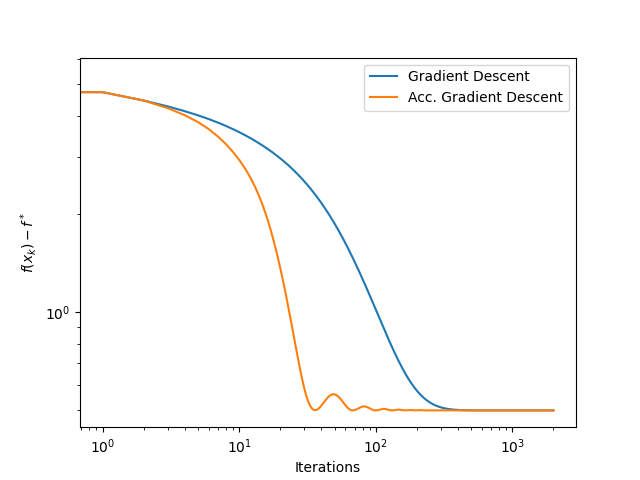
\includegraphics[width=0.45\textwidth]{img/first_order_correctness.png}
    \caption{First-order method convergence for Nesterov's difficult tensor methods ($d=25$, k=$10$, $p=1$).}
    \label{fig:nesterov_first}
\end{figure}

\begin{figure}
    \centering
    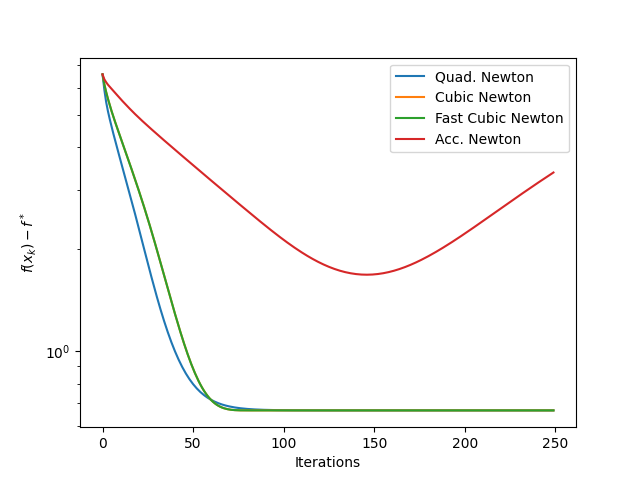
\includegraphics[width=0.45\textwidth]{img/second_order_correctness.png}
    \caption{Second-order method convergence for Nesterov's difficult tensor methods ($d=25$, k=$10$, $p=2$).}
    \label{fig:nesterov_second}
\end{figure}

There are other less direct ways we can verify our implementations. Figure~\ref{fig:ot_example} shows an example transport plan for two randomly generated marginals. Visual inspection of the plan passes several sanity checks, such as only the top right quadrant being non-zero. Another simpler sanity check was described in the fall report.

\begin{figure}
    \centering
    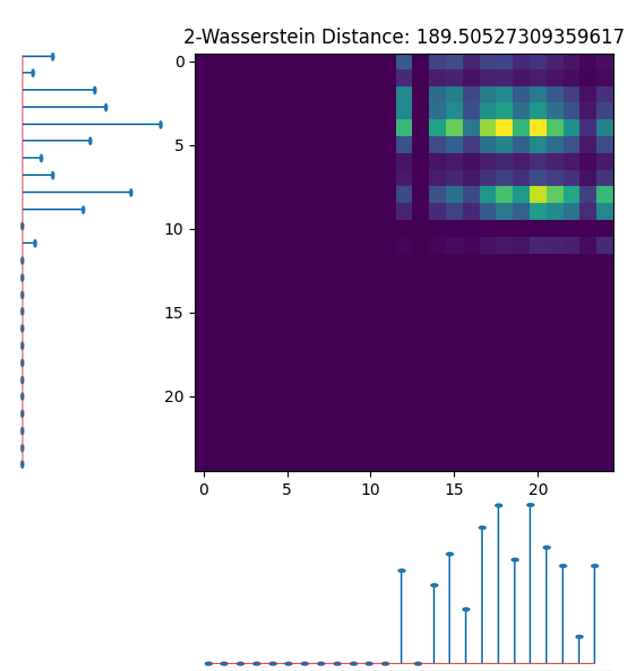
\includegraphics[width=0.45\textwidth]{img/ot.png}
    \caption{Kantorovich transport plan and $2$-Wasserstein distance computed for two example marginal distributions. This transport plan was obtained using Nesterov accelerated gradient method.}
    \label{fig:ot_example}
\end{figure}

Logistic regression can also be used to verify the correctness of these methods. The classification accuracy for methods besides hyperfast are shown in Table~\ref{tab:acc_class_libsvm}. The methods are labeled as follows: gradient descent (1), accelerated gradient descent (2), quadratically-regularized Newton method (3), cubic-regularized Newton method(4), and accelerated cubic-regularized Newton method (5). The generally good performance of the resulting binary classifier adds support to the efficacy of the implementations. Note for poorly scaled data, however, the results are poor. Note also that accelerated cubic Newton method can diverge, causing poor results (see the `australian\_scaled' column, for example).

\begin{table}[]
    \centering
    \begin{tabular}{c|ccccc}
    \textbf{Dataset} & \textbf{1} & \textbf{2} & \textbf{3} & \textbf{4} & \textbf{5} \\
    \hline
    \hline
         a9a & 0.837 & 0.849 & 0.848 & 0.849 & 0.770 \\
         australian & 0.445 & 0.445 & 0.638 & 0.443/0.434 & 0.445 \\
         australian\_scaled & 0.875 & 0.877 & 0.875 & 0.880 & 0.765 \\
         ijcnn1 & 0.903 & 0.914 & 0.908 & 0.915 & 0.908 \\
         mushrooms & 0.974 & 0.999 & 0.999 & 1.000 & 0.995 \\
         phishing & 0.921 & 0.937 & 0.930 & 0.939 & 0.915
    \end{tabular}
    \caption{Classification accuracy of various methods for different LIBSVM datasets.}
    \label{tab:acc_class_libsvm}
\end{table}

\subsection{Performance}

Figures~\ref{fig:ot_grad} and \ref{fig:libsvm_results} show the performance of first- and second-order methods for the logistic regression and optimal transport problems. The hyperfast method was only implemented for logistic regression, and it did not converge (the loss function value essentially did not change). Note that cubic regularization performs well for the logistic regression case, but not the optimal transport case.

\begin{figure}
    \centering
    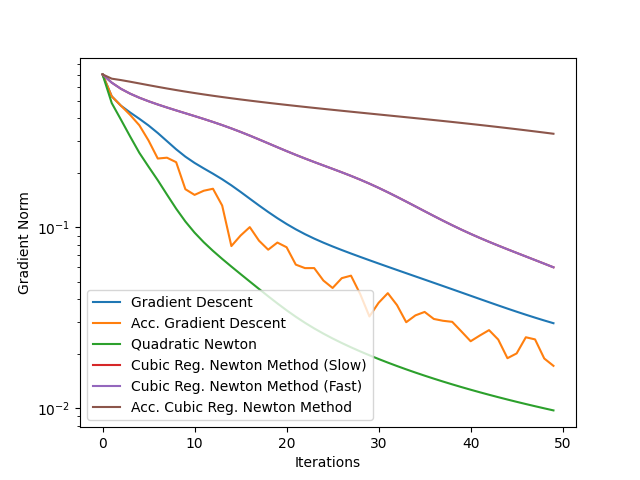
\includegraphics[width=0.45\textwidth]{img/ot_grad2.png}
    \caption{Gradient norm versus iterations for all methods excluding hyperfast on the optimal transport problem (randomly generated distributions of the form shown in Figure~\ref{fig:ot_example} in $S(25)$.}
    \label{fig:ot_grad}
\end{figure}

\begin{figure}
    \centering
    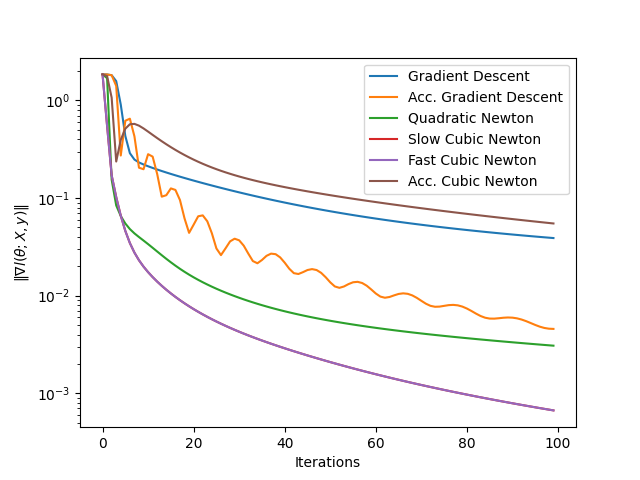
\includegraphics[width=0.45\textwidth]{img/libsvm_grad.png}
    \caption{Gradient norm versus iterations for all methods excluding hyperfast on the LIBSVM mushrooms problem.}
    \label{fig:libsvm_results}
\end{figure}

\subsection{GPU Acceleration Performance}
All supported second-order methods in Hoop3 were used to benchmark the runtime improvement associated from using the logistic regression Hessian GPU kernel. The results are shown in Figure~\ref{fig:gpu_results}. This figure shows drastic improvements associated with using the GPU, even for an unoptimized kernel that does not utilize advanced GPU concepts such as coalesced memory reads. These results are very promising and motivate future work into using GPUs to reduce the computational burden of higher order methods.

\begin{figure}
    \centering
    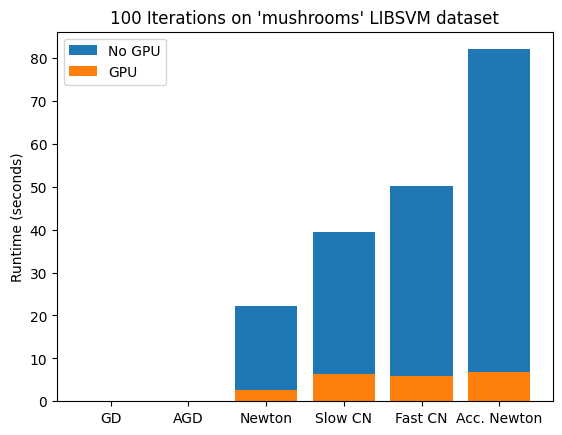
\includegraphics[width=0.45\textwidth]{img/gpu_results.png}
    \caption{Runtime improvements second-order methods solving the binary logistic regression problem on the LIBSVM mushrooms dataset. The methods were run for $100$ iterations.}
    \label{fig:gpu_results}
\end{figure}

\section{Conclusion}
\label{sec:conclusion}
In summary, while some higher-order method implementations performed well on optimal transport and logistic regression, others did not. The results of this work make clear the importance of either using extremely tight Lipschitz constants or turning to adaptive methods. Additionally, further examination into the correctness of implementation is warranted. Despite the challenges associated with implementing the accelerated cubic Newton and hyperfast methods, this project has resulted in the creation of an easy-to-use, GPU-accelerated library for higher order methods with supports for both logistic regression and optimal transport problems.

There are several future directions for this research. Our work on this project suggests the investigation of adaptive step size to eliminate issues relating to loose Lipschitz constants. Another direction is the implementation of GPU acceleration for obtaining higher-order information of the optimal transport dual. Yet another interesting direction is the distributed computation of $2$-Wasserstein barycenters, which I am investigating in ELEC 570.

\section*{Acknowledgment} \label{sec:acknowledgement}

The author would like to thank Dr. C\'esar A. Uribe for advising this research project. The author appreciates the guidance of Dr. Joseph Young, the director of the ECE master's program. The author would also like to thank the Rice Electrical and Computer Engineering department for providing a full tuition scholarship to pursue graduate studies.

\bibliographystyle{ieeetr}
\bibliography{refs}

\appendices

\section{}\label{sec:test}

In this appendix, we discuss the derivation of $L_3$ for the logistic regression loss function. First, we start by computing the fourth derivative of $f: \mathbb{R}^d \mapsto \mathbb{R}$, which is shown in Equation~\ref{eq:fourth}.

\begin{equation}
    \frac{\partial d^4 f}{\partial \theta_w \partial \theta_j \partial \theta_k \partial \theta_l} = \frac{1}{N} \sum_{i=1}^N X_{ik} X_{il} X_{ij} X_{iw} g(z_i)
    \label{eq:fourth}
\end{equation}

\begin{equation}
    g(z_i) = \frac{(e^{-z_i} - 3e^{-3 z_i})(1 + e^{-z_i}) - 4e^{-z_i} (e^{-z_i} - e^{-3z_i})}{(1+e^{-z_i})^5}
\end{equation}

\begin{equation}
    z_i = y_i \mathbf{x_i}^T \mathbf{\theta}
\end{equation}

By visual inspection with the Desmos graphing tool, $|g(z_i)| \le \frac{1}{8}$. Let us denote $A$ as the fourth-order tensor of $f$. Note that $\|A\|_2 \le \|A\|_F$ since the induced two-norm of a tensor is less than the Frobenius norm of said tensor (this assumes the matrix case~\cite{frobenius} generalizes). Since the induced two-norm of the fourth-order tensor appears to be bounded above by $\|A\|_F$, this bounds the third-order Lipschitz constant of the third-order tensor. Therefore, we arrive at the third-order Lipschitz constant for logistic regression shown in Equation~\ref{eq:l3}.

\begin{equation}
    L_3 = \frac{1}{8N} \sqrt{\sum_{w, j, k, l = 1}^d \sum_{i=1}^N \left(X_{ik} X{il} X_{ij} X_{iw} \right)^2}
    \label{eq:l3}
\end{equation}

This constant, however, takes a very long to compute, especially if $d$ or $N$ are large, which they usually are. Therefore, we suggest adaptive methods as an alternative.


\end{document}
